\section{Thiết kế DataWarehouse Schema}
\subsection{Quá trình thiết kế}
\subsubsection{Thiết kế DW Schema theo lý thuyết, góc nhìn cá nhân/chủ quan về giao thông}

Giai đoạn khởi đầu của quá trình thiết kế kho dữ liệu được thực hiện dựa trên cơ sở lý thuyết nền tảng của mô hình hóa dữ liệu đa chiều theo trường phái Kimball, kết hợp với những quan sát trực quan về hoạt động giao thông đô thị.

Ở bước này, mục tiêu chủ đạo là xác định các thành phần cốt lõi của hệ thống dữ liệu, bao gồm: Quy trình nghiệp vụ (Business Processes), Hạt dữ liệu (Grain), Các chiều phân tích (Dimensions) và Các bảng sự kiện (Fact Tables). Đây là bước định hình khung sườn ban đầu để hình thành kiến trúc Data Warehouse.

Tuy nhiên, do chưa tham chiếu sâu các tiêu chuẩn kỹ thuật chuyên ngành về cầu đường, tổ chức giao thông, và mô hình hóa mạng lưới giao thông, bản thiết kế sơ khai mang màu sắc thiên về lý thuyết, thiếu sự tinh chỉnh theo các yêu cầu nghiệp vụ thực tiễn. Điều này dẫn tới việc hình thành các lược đồ sao (Star Schema) rời rạc, các bảng chiều thiếu chức năng mô tả đầy đủ và chưa đạt tính tối ưu về mặt ngữ nghĩa.

\subsubsubsection{Tiếp cận mô hình Star Schema độc lập}
Dựa trên các nguyên tắc cơ bản của thiết kế Data Warehouse, nhóm nghiên cứu đã khởi đầu bằng cách phân tách các quy trình nghiệp vụ riêng biệt thành các lược đồ sao độc lập. Tư duy thiết kế ở giai đoạn này hướng vào việc giải quyết từng câu hỏi phân tích đơn lẻ, chưa tính đến nhu cầu tích hợp dữ liệu thành một kiến trúc tổng thể.

Hai hướng tiếp cận chính được hình thành:
\begin{enumerate}
    \item \textbf{Lược đồ lưu lượng giao thông (Traffic Flow Schema):} Mục tiêu là trả lời câu hỏi: “Có bao nhiêu phương tiện đã di chuyển qua một vị trí, tuyến hoặc phân đoạn đường trong một khoảng thời gian nhất định?”. Bảng Fact chủ đạo chứa dữ liệu đếm xe, liên kết với các bảng Dim cơ bản (thời gian, vị trí, loại phương tiện).
    \item \textbf{Lược đồ sự cố giao thông (Incident Schema):} Tập trung giải quyết câu hỏi: “Sự cố giao thông xảy ra ở đâu và khi nào?”. Bảng Fact chứa thông tin va chạm/sự cố, kết nối với chiều thời gian, vị trí và loại sự cố.
\end{enumerate}

\begin{figure}[H]
    \centering
    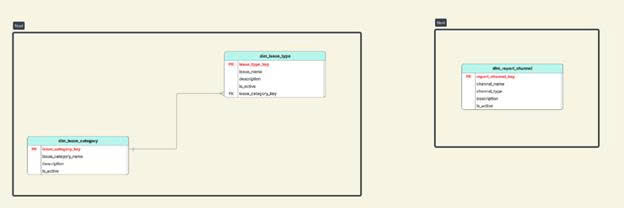
\includegraphics[width=0.9\textwidth]{Images/Picture1}
    \vspace{6mm}
    \caption{Các lược đồ Star Schema ban đầu}
\end{figure}

Cách tiếp cận theo mô hình Star Schema tách biệt này vô tình tạo nên các “ốc đảo dữ liệu” (data silos). Các bảng Dimension được tạo dựng độc lập theo từng Fact, dẫn đến tình trạng thiếu các Dimension chuẩn hóa, dùng chung. Điều này hạn chế khả năng thực hiện các phân tích đa chiều tổng hợp, đặc biệt là các phân tích chéo giữa lưu lượng giao thông và sự cố – vốn là yêu cầu quan trọng đối với bài toán ra quyết định trong thực tế.

\subsubsubsection{Thiết kế các bảng Dimension dựa trên quan sát chủ quan}
Do hạn chế về kiến thức chuyên ngành trong giai đoạn đầu, các bảng Dimension được xây dựng chủ yếu dựa trên suy luận trực quan hoặc kinh nghiệm phổ quát, thay vì trên nền tảng các quy chuẩn kỹ thuật của lĩnh vực giao thông vận tải. Điều này dẫn đến việc giản lược quá mức các thành phần mô tả, khiến các bảng chiều thiếu khả năng phản ánh đầy đủ hiện trạng vận hành giao thông.
\vspace{2mm}
Một số hạn chế điển hình bao gồm:
\\
\textbf{1. Chiều Không gian – dim\_location}
\begin{itemize}
    \item \textit{Cách tiếp cận ban đầu:} Vị trí giao thông được xem đơn thuần là một điểm địa lý (Kinh độ/Vĩ độ).
    \item \textit{Hạn chế:} Bỏ qua cấu trúc mạng lưới giao thông (Tuyến đường, Phân đoạn, Hướng lưu thông, Lý trình). Dẫn đến không thể phân tích hiện tượng ùn tắc theo chiều dài tuyến. Không thể mô tả sự khác biệt giữa hai làn đường khác nhau tại cùng tọa độ. Khó khăn trong việc đồng bộ dữ liệu từ nhiều nguồn (GPS, camera, cảm biến).

\end{itemize}

\begin{figure}[H]
    \centering
    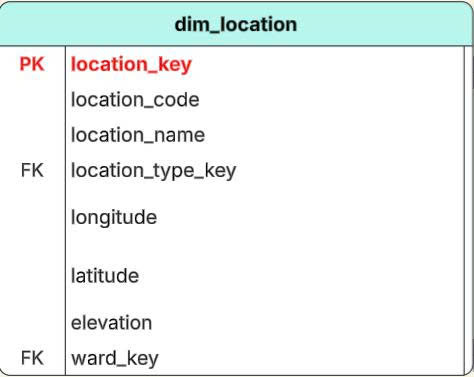
\includegraphics[width=0.5\textwidth]{Images/Picture2}
    \vspace{6mm}
    \caption{Thiết kế bảng dim\_location ban đầu}
\end{figure}

\textbf{2. Chiều Thời gian – dim\_time}
\begin{itemize}
    \item \textit{Cách tiếp cận ban đầu:} Xây dựng theo lịch dương (Giờ, Ngày, Tháng, Năm).
    \item \textit{Hạn chế:} Không phản ánh được thuộc tính đặc thù giao thông như: Giờ cao điểm/thấp điểm, Giờ cấm tải, Các ngày lễ/sự kiện, Yếu tố mùa vụ.
\end{itemize}

\begin{figure}[H]
    \centering
    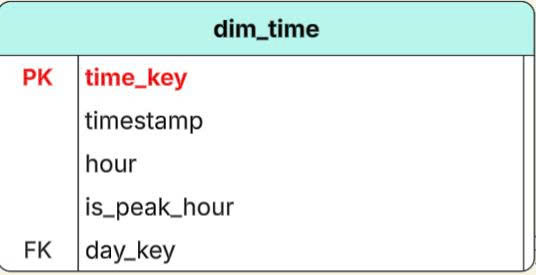
\includegraphics[width=0.5\textwidth]{Images/Picture3}
    \vspace{6mm}
    \caption{Thiết kế bảng dim\_time ban đầu}
\end{figure}

\textbf{3. Chiều Phương tiện – dim\_vehicle}
\begin{itemize}
    \item \textit{Cách tiếp cận ban đầu:} Phân loại theo tên gọi phổ biến (Xe máy, Ô tô...).
    \item \textit{Hạn chế:} Thiếu các thông số kỹ thuật (Số trục, Tải trọng, Kích thước, Hệ số PCU) cần thiết cho mô hình dự báo.
\end{itemize}

\begin{figure}[H]
    \centering
    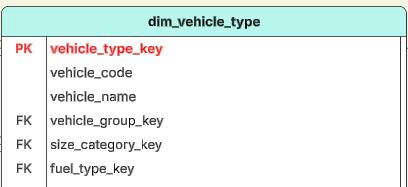
\includegraphics[width=0.5\textwidth]{Images/Picture4}
    \vspace{6mm}
    \caption{Thiết kế bảng dim\_vehicle\_type ban đầu}
\end{figure}

\subsubsubsection{Kết luận về thiết kế sơ khởi}
Thiết kế ban đầu tuy tuân thủ lý thuyết Fact-Dimension nhưng thiếu chiều sâu nghiệp vụ, tạo ra 3 hạn chế cốt lõi:
\begin{itemize}
    \item Thiếu tính liên kết giữa các quy trình nghiệp vụ (không có Dimension dùng chung).
    \item Dữ liệu mô tả nghèo nàn, thiếu phân cấp (không hỗ trợ drill-down sâu).
    \item Khả năng mở rộng thấp (khó tích hợp đa nguồn GPS/Camera).
\end{itemize}

\subsubsection{Phân tích nghiệp vụ nâng cao và xây dựng mô hình Galaxy Schema}

Sau khi nhận diện bất cập, nhóm nghiên cứu chuyển sang phân tích nghiệp vụ chuyên sâu và đề xuất mô hình \textbf{Galaxy Schema} – phù hợp khi nhiều quy trình nghiệp vụ chia sẻ chung một tập các bảng chiều chuẩn hóa.

\subsubsubsection{Phân tích ma trận nghiệp vụ}
Thông qua việc phân tích các nhóm nghiệp vụ từ BKTraffic, tài liệu liên quan, nhóm nhận thấy các luồng dữ liệu giao thông không tồn tại độc lập mà có mối quan hệ chặt chẽ với nhau. Các câu hỏi phân tích thực tế thường yêu cầu kết hợp dữ liệu từ nhiều nguồn khác nhau. Điều này làm nổi bật nhu cầu thiết kế mô hình dữ liệu tích hợp thay vì các Star Schema tách biệt.

\begin{table}[H]
\centering
\caption{Ma trận quy trình nghiệp vụ và các chiều dữ liệu}
\begin{tabular}{|l|c|c|c|c|c|c|}
\hline
\textbf{Quy trình nghiệp vụ} & \textbf{Time} & \textbf{Location} & \textbf{Vehicle} & \textbf{Weather} & \textbf{Incident} & \textbf{Source} \\ \hline
Theo dõi lưu lượng & X & X & X & X & & X \\ \hline
Giám sát sự cố & X & X & & X & X & X \\ \hline
Vận tải công cộng & X & X & X & & & \\ \hline
Dự báo thời tiết & X & X & & X & & \\ \hline
Điều phối tín hiệu & X & X & & & & X \\ \hline
\end{tabular}
\end{table}

Một số mối liên kết nghiệp vụ tiêu biểu:
\begin{itemize}
    \item Mối liên hệ giữa lưu lượng và an toàn giao thông\\
    Các nghiệp vụ như “Dự báo ùn tắc đa yếu tố” và “Đánh giá rủi ro theo khu vực” yêu cầu đồng thời thông tin về mật độ lưu thông (từ fact\_traffic\_flow) và thông tin sự cố, tai nạn (từ fact\_incident). Đây là dạng phân tích phức hợp, không thể thực hiện hiệu quả khi hai hệ thống tồn tại độc lập.
    \item Mối liên hệ giữa vận hành giao thông và yếu tố môi trường \\
    Nghiệp vụ “Dự báo giao thông theo điều kiện khí hậu” đòi hỏi tích hợp dữ liệu mưa, nhiệt độ, sương mù từ nguồn thời tiết (fact\_external\_condition) để giải thích sự biến động của tốc độ dòng xe hoặc mức độ ùn ứ.
    \item Mối liên hệ giữa sự kiện và nhu cầu giao thông\\
    Nghiệp vụ “Dự báo mật độ quanh khu vực sự kiện” yêu cầu liên kết dữ liệu về sự kiện đô thị (fact\_event) với hạ tầng giao thông, tuyến đường, phân đoạn và mật độ tại từng khu vực.

\end{itemize}

Kết quả phân tích cho thấy cần xây dựng tập Conformed Dimensions dùng chung để xóa bỏ tình trạng “ốc đảo dữ liệu”, đảm bảo các bảng fact có thể truy vấn và kết hợp dữ liệu đồng nhất.

\subsubsubsection{Tái thiết kế các Conformed Dimensions}

Để xử lý được các nghiệp vụ đa chiều và phức hợp, các bảng Dimension được tái cấu trúc với mức độ chuẩn hóa và hàm chứa ngữ nghĩa cao hơn đáng kể so với giai đoạn thiết kế ban đầu.\\

\textbf{1. Nhóm chiều Thời gian:}
Cung cấp trục thời gian đa cấp độ, liên kết toàn bộ các bảng Fact.
\begin{itemize}
    \item \texttt{dim\_date}, \texttt{dim\_date\_time}: Trục thời gian lịch và timestamp thực.
    \item \texttt{dim\_time\_of\_day}: Mô tả chi tiết 1.440 phút trong ngày, hỗ trợ bucket (5', 15').
    \item \texttt{dim\_shift}: Quản lý ca làm việc, giờ cao điểm.
    \item \texttt{dim\_holiday}, \texttt{bridge\_date\_holiday}: Quản lý ngày lễ, sự kiện đặc biệt.
\end{itemize}

\textbf{2. Nhóm chiều Không gian \& Hạ tầng:}
Hệ tọa độ chung mô tả cấu trúc phân cấp mạng lưới.
\begin{itemize}
    \item \texttt{dim\_segment}: Đơn vị cơ bản (phân đoạn đường giữa 2 node).
    \item \texttt{dim\_node}: Các nút giao, giao lộ.
    \item \texttt{dim\_route}, \texttt{bridge\_route\_segment}: Lộ trình và thứ tự segment.
    \item \texttt{dim\_way}, \texttt{dim\_road}: Cấp độ tuyến đường, trục chính.
\end{itemize}

\textbf{3. Nhóm chiều Đối tượng tham gia:}
\begin{itemize}
    \item \texttt{dim\_user}, \texttt{dim\_user\_detail}: Định danh và thuộc tính người dùng (SCD).
    \item \texttt{dim\_vehicle\_type}: Chuẩn hóa danh mục phương tiện (PCU, khí thải...).
\end{itemize}

\textbf{4. Nhóm chiều Ngữ cảnh \& Sự cố:}
\begin{itemize}
    \item \texttt{dim\_incident\_type}: Phân loại sự cố (tai nạn, ngập, công trình).
    \item \texttt{dim\_response\_unit}: Lực lượng phản ứng.
    \item \texttt{dim\_weather}: Thời tiết thực tế (mưa, gió, tầm nhìn).
\end{itemize}

\subsubsubsection{Thiết kế các bảng Fact theo nghiệp vụ}
Toàn bộ kiến trúc được tổ chức theo mô hình Galaxy Schema với 4 cụm nghiệp vụ:

\begin{itemize}
    \item \textbf{Cụm Vận hành Giao thông:}
    \begin{itemize}
        \item \texttt{fact\_traffic\_flow}: Lưu lượng tổng hợp, tốc độ trung bình, mức độ tắc nghẽn.
        \item \texttt{fact\_traffic\_flow\_by\_vehicle}: Lưu lượng chi tiết theo loại xe.
    \end{itemize}
    
    \item \textbf{Cụm Hành vi Người dùng:}
    \begin{itemize}
        \item \texttt{fact\_user\_travel\_time}: Hiệu suất di chuyển từng chuyến đi.
        \item \texttt{fact\_user\_mobility}: Thống kê hành vi tổng hợp.
    \end{itemize}
    
    \item \textbf{Cụm An toàn \& Sự cố:}
    \begin{itemize}
        \item \texttt{fact\_incident}: Ghi nhận sự cố, thời gian xử lý, mức độ nghiêm trọng.
    \end{itemize}
    
    \item \textbf{Cụm Hiệu quả Hệ thống:}
    \begin{itemize}
        \item \texttt{fact\_route\_recommendation}: Đánh giá hiệu quả gợi ý tuyến đường.
    \end{itemize}
\end{itemize}

\subsubsubsection{Tổng quan quá trình chuyển đổi}
Quá trình thiết kế là sự chuyển dịch từ: \textbf{Star Schema} (đơn giản, rời rạc) $\rightarrow$ \textbf{Snowflake Schema} (chuẩn hóa chiều không gian để phản ánh đúng topo mạng lưới) $\rightarrow$ \textbf{Galaxy Schema} (tích hợp đa luồng nghiệp vụ trên cùng hệ thống Dimension).



\subsubsection{Phân tích tính khả thi}
Phần này tập trung tìm hiểu và phân tích các nguồn data input, bao gồm 3 nguồn chính sau: TomTom, Google Maps và OpenStreetMap để xác thực độ khả thi của thiết kế tại mục 5.1.2, qua đó điều chỉnh để tính khả thi đạt 100\%.

\subsubsubsection{TomTom}

\textbf{Các loại dữ liệu và phạm vi cung cấp:} TomTom cung cấp một hệ sinh thái dữ liệu giao thông toàn diện, bao gồm cả dữ liệu thời gian thực (Real-time) với tần suất cập nhật mỗi phút và dữ liệu lịch sử phục vụ thống kê. Các nhóm dữ liệu chính bao gồm:
\begin{itemize}
    \item \textbf{Dữ liệu dòng giao thông (Traffic Flow):} Cung cấp các chỉ số về tốc độ quan sát thực tế (observed speed), thời gian di chuyển (travel time) và so sánh với tốc độ dòng chảy tự do (free-flow) cho từng phân đoạn đường (road segments).
    \item \textbf{Sự cố giao thông (Traffic Incidents):} Thông tin chi tiết về các sự kiện gây cản trở giao thông như tai nạn, công trường thi công, hoặc đường đóng. Dữ liệu bao gồm vị trí bắt đầu/kết thúc, độ dài đoạn ảnh hưởng, loại sự cố và mức độ nghiêm trọng.
    \item \textbf{Dữ liệu hiển thị và điều khiển:} Hỗ trợ các lớp bản đồ Vector Tiles cho luồng giao thông và sự cố, cùng với thông tin cập nhật giới hạn tốc độ động (Live speed restrictions) giúp tăng cường độ chính xác cho các ứng dụng dẫn đường.
\end{itemize}

\textbf{Cấu trúc và định dạng dữ liệu kỹ thuật:} Về mặt kỹ thuật, TomTom sử dụng các chuẩn dữ liệu phổ biến để đảm bảo tính tương thích cao.
\begin{itemize}
    \item Các phản hồi từ REST API (như thông tin sự cố, metadata, lỗi) được trả về dưới định dạng \textbf{JSON} tiêu chuẩn.
    \item Đối với các dữ liệu yêu cầu hiệu năng hiển thị cao như Flow/Incident Tiles, TomTom sử dụng định dạng vector nhị phân (\textbf{Binary Protobuf/PBF-like}), được tuần tự hóa bởi Google Protocol Buffers theo schema riêng.
    \item Các trường thông tin (key fields) quan trọng phục vụ cho việc mô hình hóa dữ liệu bao gồm: tọa độ không gian (\texttt{start/endLocation}), tên đường (\texttt{roadName}), tham số giao thông (\texttt{delay}, \texttt{speedObserved}, \texttt{speedFreeFlow}), độ tin cậy của dữ liệu (\texttt{confidence}) và nhãn thời gian (\texttt{timestamp}).
\end{itemize}

\textbf{Cơ chế truy cập và Chính sách sử dụng:} Để tích hợp vào hệ thống, nhà phát triển cần đăng ký API Key thông qua TomTom Developer Portal. Dữ liệu được truy xuất thông qua các RESTful API endpoints (như Traffic Incidents service) hoặc Vector Tile endpoints.
\begin{itemize}
    \item Về mặt giới hạn và chi phí, TomTom áp dụng mô hình giới hạn truy cập (Rate limits) dựa trên từng khóa API hoặc gói dịch vụ cụ thể.
    \item Mô hình chi phí dựa trên mức độ sử dụng (pay-as-you-go). Đáng chú ý, độ trễ dữ liệu (latency) được duy trì ở mức thấp, cập nhật từng phút, phù hợp cho các bài toán điều hướng thời gian thực.
\end{itemize}

\textbf{Đánh giá khả năng ứng dụng tại TP.HCM:}
\begin{itemize}
    \item \textbf{Ưu điểm:} Dữ liệu có độ tin cậy cao, cập nhật nhanh (real-time), hỗ trợ Vector Tiles giúp việc hiển thị và streaming dữ liệu lên bản đồ số mượt mà, hiệu quả. Đây là nguồn dữ liệu lý tưởng cho các ứng dụng yêu cầu độ chính xác cao như điều phối xe hoặc dẫn đường.
    \item \textbf{Nhược điểm và Thách thức:} Chi phí vận hành có thể tăng cao khi mở rộng quy mô (scale). Ngoài ra, độ phủ sóng dữ liệu (coverage) của TomTom tại TP.HCM chủ yếu tập trung tốt ở các đô thị lớn và đường trục chính; đối với hệ thống đường hẻm, đường nhánh nhỏ đặc thù của Việt Nam, lượng dữ liệu từ cảm biến/probe data có thể ít hơn.
\end{itemize}

\textbf{Kết luận:} Để tối ưu hóa hiệu quả và chi phí cho dự án, chiến lược đề xuất là chỉ sử dụng dữ liệu TomTom cho các tuyến đường trục chính, đường huyết mạch có vai trò quan trọng trong việc điều tiết giao thông toàn thành phố. Đối với các tuyến đường nhỏ hoặc hẻm không có tác động lớn đến luồng giao thông tổng thể, hệ thống sẽ cân nhắc sử dụng các nguồn dữ liệu thay thế.

\subsubsubsection{Google Maps}

\textbf{Các loại dữ liệu và phạm vi cung cấp:} Google Maps Platform cung cấp hệ sinh thái dữ liệu giao thông tập trung mạnh vào trải nghiệm dẫn đường và trực quan hóa.
\begin{itemize}
    \item \textbf{Dữ liệu giao thông thời gian thực (Real-time Traffic):} Cung cấp lớp hiển thị trực quan (\texttt{TrafficLayer}) trên bản đồ thông qua Maps JavaScript API.
    \item \textbf{Định tuyến và thời gian di chuyển (Traffic-aware Routing):} Thông qua \textbf{Directions API} và \textbf{Routes API} (\texttt{ComputeRoutes}), cung cấp ước lượng thời gian di chuyển chính xác dựa trên tình trạng giao thông thực tế.
    \item \textbf{Dữ liệu hạ tầng đường bộ:} \textbf{Roads API} hỗ trợ các tính năng như bám đường (snap-to-road), truy xuất giới hạn tốc độ (speed limits).
    \item \textbf{Lưu ý về sự cố giao thông:} Khác với TomTom, Google không cung cấp một luồng dữ liệu (feed) riêng biệt và có cấu trúc cho các sự cố (tai nạn, công trường) qua REST API.
\end{itemize}

\textbf{Cấu trúc và định dạng dữ liệu kỹ thuật:}
\begin{itemize}
    \item Các phản hồi từ REST API được trả về dưới định dạng \textbf{JSON}.
    \item Các trường thông tin quan trọng bao gồm: thời gian di chuyển trong điều kiện giao thông (\texttt{duration\_in\_traffic}), mô hình giao thông (\texttt{traffic\_model}), hình học tuyến đường (\texttt{geometry polyline}), phân đoạn hành trình (\texttt{legs/steps}) và giới hạn tốc độ (\texttt{speedLimits}).
    \item Dữ liệu có độ trễ thấp, phù hợp cao cho các tác vụ thời gian thực.
\end{itemize}

\textbf{Cơ chế truy cập và Chính sách sử dụng:} Việc truy cập dữ liệu được quản lý chặt chẽ thông qua Google Cloud Console, yêu cầu bắt buộc phải có API Key và tài khoản thanh toán (Billing account). Chi phí tính theo mô hình pay-as-you-go, khá cao cho các tính năng nâng cao như \texttt{ComputeRoutes} ở quy mô lớn.

\textbf{Đánh giá khả năng ứng dụng tại TP.HCM:}
\begin{itemize}
    \item \textbf{Ưu điểm:} Độ phủ dữ liệu (coverage) tại TP.HCM rất tốt nhờ lượng người dùng thiết bị di động khổng lồ. Khả năng tích hợp sâu với các SDK (Mobile, Web) hỗ trợ mạnh mẽ cho các bài toán định tuyến.
    \item \textbf{Nhược điểm và Thách thức:} Rào cản lớn nhất là \textbf{chi phí vận hành}. Mô hình tính phí trên mỗi yêu cầu (request-based) tạo ra gánh nặng tài chính lớn khi thu thập dữ liệu liên tục cho Data Warehouse. Ngoài ra, việc thiếu API cung cấp dữ liệu sự cố dưới dạng cấu trúc gây khó khăn cho việc thống kê tự động.
\end{itemize}

\textbf{Kết luận:} Do các hạn chế về chi phí và cấu trúc dữ liệu sự cố, Google Maps Platform được xếp độ \textbf{ưu tiên thấp nhất} trong việc làm nguồn dữ liệu đầu vào cho Kho dữ liệu. Nguồn này sẽ chỉ được cân nhắc sử dụng cho các chức năng hiển thị (Visual layer) ở phía người dùng cuối.

\subsubsubsection{OpenStreetMap}

\textbf{Các loại dữ liệu và phạm vi cung cấp:} OpenStreetMap (OSM) là cơ sở dữ liệu bản đồ nguồn mở toàn cầu. OSM cung cấp nền tảng dữ liệu địa lý tĩnh phong phú (mạng lưới đường bộ, ranh giới hành chính, POIs). Tuy nhiên, hệ thống \textbf{không cung cấp sẵn} dữ liệu lưu lượng giao thông thời gian thực hay thông tin sự cố tức thời.

\textbf{Cấu trúc và định dạng dữ liệu kỹ thuật:}
\begin{itemize}
    \item Dữ liệu OSM được tổ chức linh hoạt dựa trên mô hình thẻ (tags).
    \item Sử dụng \textbf{PBF (Protocolbuffer Binary Format)} cho lưu trữ offline và \textbf{OSM XML} hoặc \textbf{Overpass JSON} cho API.
    \item Các trường thông tin quan trọng: loại đường (\texttt{highway}), giới hạn tốc độ (\texttt{maxspeed}), chiều di chuyển (\texttt{oneway}), số làn xe (\texttt{lanes}), kết cấu mặt đường (\texttt{surface}).
\end{itemize}

\textbf{Cơ chế truy cập và Chính sách sử dụng:} OSM cung cấp cơ chế truy cập rất linh hoạt và mở (thông qua Geofabrik hoặc Overpass API). Dữ liệu hoàn toàn miễn phí dưới giấy phép \textbf{ODbL}. Chi phí thực tế chuyển dịch sang phần hạ tầng kỹ thuật (self-host) để tránh giới hạn truy cập.

\textbf{Đánh giá khả năng ứng dụng tại TP.HCM:}
\begin{itemize}
    \item \textbf{Ưu điểm:} Thế mạnh lớn nhất là độ chi tiết về hình học đường bộ, đặc biệt là hệ thống \textbf{đường hẻm, ngõ nhỏ} và lối đi bộ. Đây là nguồn dữ liệu nền tảng tuyệt vời để xây dựng đồ thị giao thông (topology graph).
    \item \textbf{Nhược điểm:} Thiếu dữ liệu traffic thời gian thực, không thể dùng độc lập để dự báo tắc nghẽn. Độ đồng nhất của dữ liệu thuộc tính tại ngoại ô có thể không cao.
\end{itemize}

\textbf{Kết luận:} OpenStreetMap là giải pháp tối ưu để giải quyết bài toán "phủ sóng" bản đồ tại các khu vực hẻm nhỏ của TP.HCM. Chiến lược đề xuất là sử dụng OSM làm \textbf{lớp bản đồ nền (Base Map)} và mạng lưới định tuyến cơ sở.

% Bảng so sánh
\begin{table}[H]
\centering
\caption{Bảng tóm tắt so sánh 3 nguồn dữ liệu}
\begin{tabular}{|p{3cm}|p{4cm}|p{4cm}|p{4cm}|}
\hline
\textbf{Tiêu chí} & \textbf{TomTom} & \textbf{Google Maps Platform} & \textbf{OpenStreetMap (OSM)} \\ \hline
Độ phủ (TP.HCM) & Rộng, commercial-grade; đường chính tốt. & Rất rộng; coverage cao ở đô thị lớn. & Geometries \& POI tốt ở khu vực cộng đồng active; mạnh về hẻm/chi tiết nhỏ. \\ \hline
Độ chính xác & Cao cho road attributes \& traffic metrics trên đường lớn. & Rất cao; enterprise-grade map + signals từ user base lớn. & Rất tốt về geometry; attribute completeness biến thiên. \\ \hline
Real-time & \textbf{Có} — real-time flow \& incident feeds (vector tiles). & \textbf{Có} — traffic-aware routing, TrafficLayer; không có incident feed công khai. & \textbf{Không} native. Cần tích hợp bên thứ ba. \\ \hline
Chi phí & Commercial — tốn phí tùy volume; pricing theo API. & Commercial — pay-as-you-go; tốn kém ở scale lớn. & \textbf{Miễn phí} (ODbL). Chi phí ở hạ tầng (hosting). \\ \hline
\end{tabular}
\end{table}

\textbf{Kiến nghị chiến lược triển khai nguồn dữ liệu thực tiễn cho TP.HCM:}
\begin{enumerate}
    \item \textbf{Lựa chọn nguồn dữ liệu cho các tác vụ thời gian thực:} Ưu tiên sử dụng \textbf{TomTom} (cho backend/data warehouse nhờ cấu trúc dữ liệu rõ ràng) hoặc \textbf{Google Maps} (cho frontend/client-side).
    \item \textbf{Chiến lược tự chủ dữ liệu và tối ưu chi phí:} Sử dụng \textbf{OpenStreetMap (OSM)} làm lớp bản đồ nền cơ sở (Base Map) để giải quyết bài toán ngân sách và đặc thù mạng lưới hẻm nhỏ.
    \item \textbf{Lộ trình kiểm thử và đánh giá tính khả thi:} Thực hiện A/B Testing và Proof of Concept (PoC) tại 1-2 quận trọng điểm để đánh giá chi phí và độ chính xác thực tế trước khi scale.
\end{enumerate}

\subsection{Kết quả}
\subsubsection{Tổng quan toàn bộ Galaxy Schema}
Mô hình Galaxy được xây dựng bằng cách sử dụng chung một tập hợp Dimensions chuẩn hóa. Tất cả các bảng Fact đều liên kết tới các Dimensions trong các chủ đề thời gian, không gian – hạ tầng, đối tượng tham gia và ngữ cảnh – sự cố, hình thành một cấu trúc phân tích đa chiều thống nhất.

\begin{figure}[H]
    \centering
    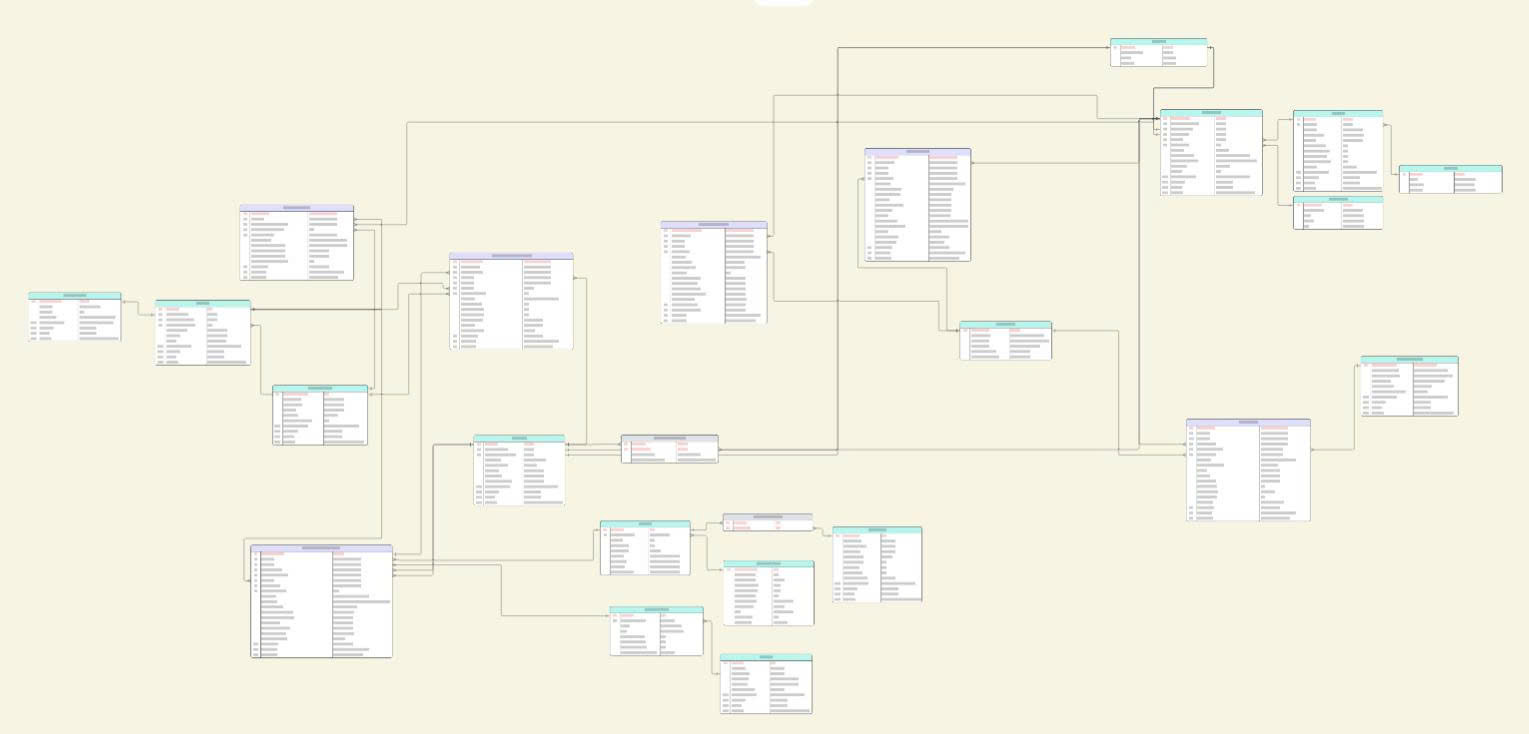
\includegraphics[width=1.0\textwidth]{Images/Picture5}
    \vspace{6mm}
    \caption{Mô hình Galaxy Schema hoàn chỉnh}
\end{figure}

\textbf{Các thành phần chính của hệ thống:}
\begin{itemize}
    \item \textbf{Hệ trục thời gian:} Bao trùm tất cả các Fact, hỗ trợ phân tích từ vi mô (phút) đến vĩ mô (năm).
    \item \textbf{Hệ tọa độ không gian – hạ tầng:} Cung cấp chuẩn tham chiếu không gian nhất quán (Segment $\rightarrow$ Node $\rightarrow$ Way $\rightarrow$ Road).
    \item \textbf{Hệ tham chiếu người dùng – phương tiện:} Phục vụ phân tích hành vi và tối ưu lộ trình.
    \item \textbf{Hệ ngữ cảnh – sự cố:} Then chốt trong phân tích an toàn và tác động môi trường.
\end{itemize}

Cách tổ chức này đảm bảo tính nhất quán dữ liệu, tăng khả năng phân tích chéo và sẵn sàng mở rộng cho các nguồn dữ liệu IoT trong tương lai.

\subsubsection{Bảng Fact}
Các ảnh bảng Fact với đầy đủ kết nối đến bảng Dim.

\begin{figure}[H]
    \centering
    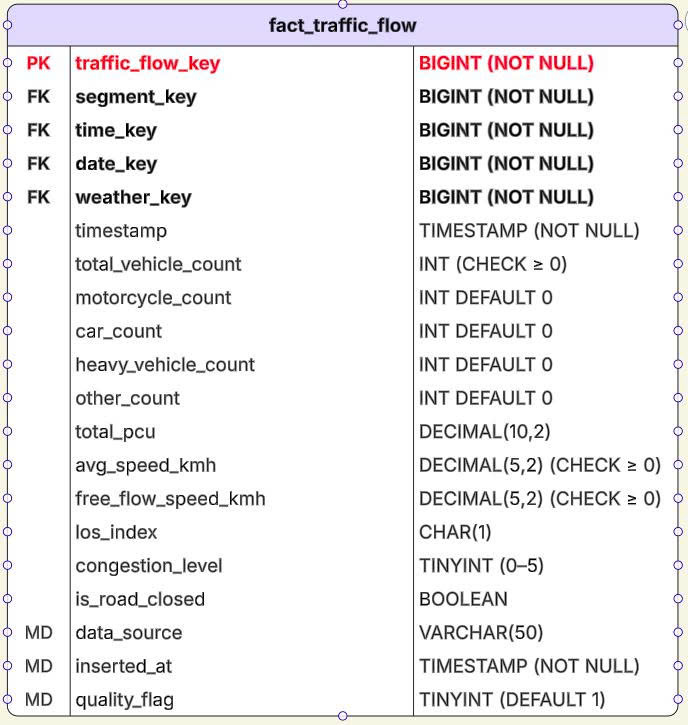
\includegraphics[width=1.0\textwidth]{Images/Picture6}
    \vspace{6mm}
    \caption{Bảng fact\_travel\_flow}
\end{figure}

\begin{figure}[H]
    \centering
   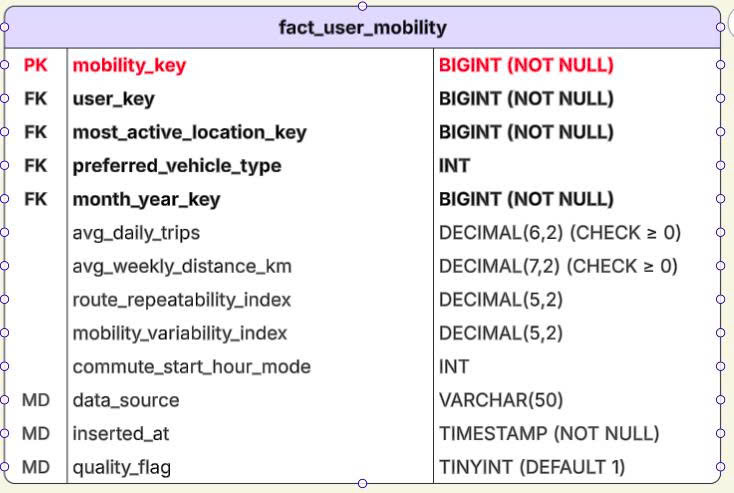
\includegraphics[width=1.0\textwidth]{Images/Picture7}
    \vspace{6mm}
    \caption{Bảng fact\_user\_mobility}
\end{figure}

\begin{figure}[H]
    \centering
    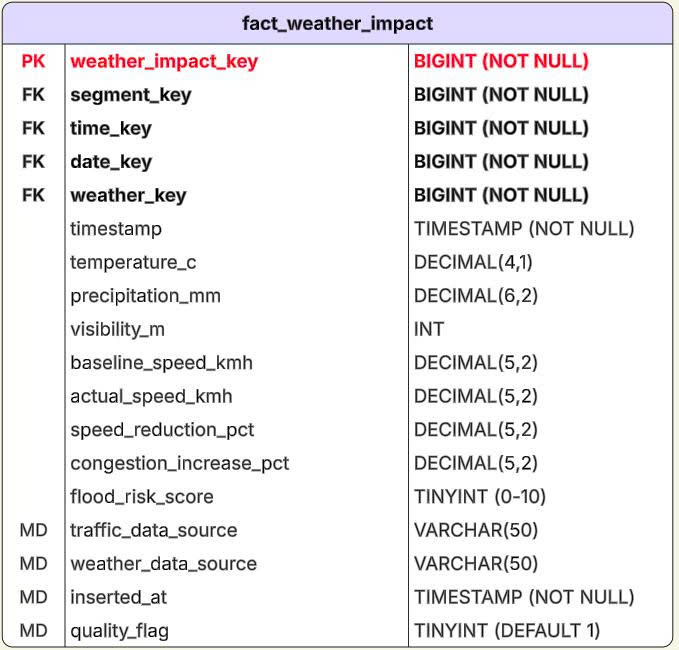
\includegraphics[width=1.0\textwidth]{Images/Picture8}
    \vspace{6mm}
    \caption{Bảng fact\_weather\_impact}
\end{figure}

\begin{figure}[H]
    \centering
   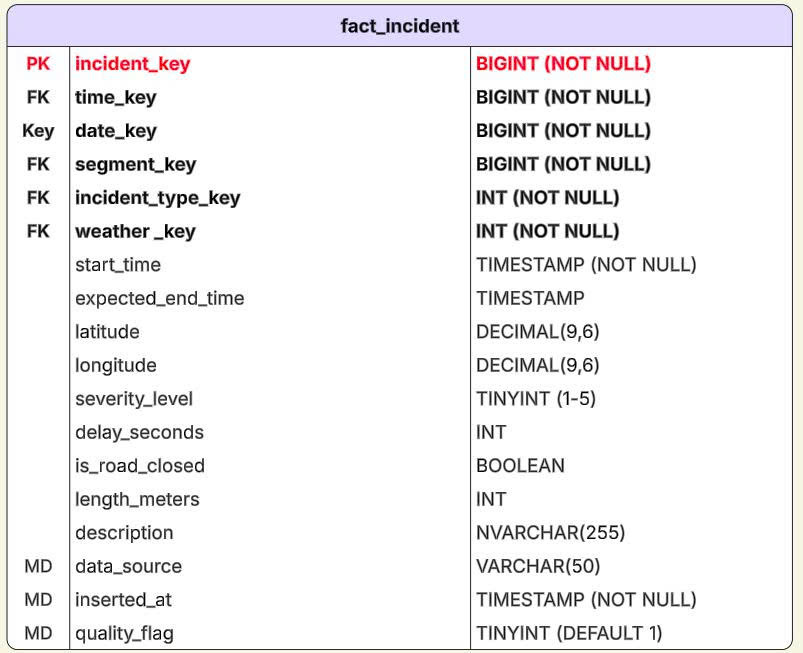
\includegraphics[width=1.0\textwidth]{Images/Picture9}
    \vspace{6mm}
    \caption{Bảng fact\_incident}
\end{figure}

\begin{figure}[H]
    \centering
    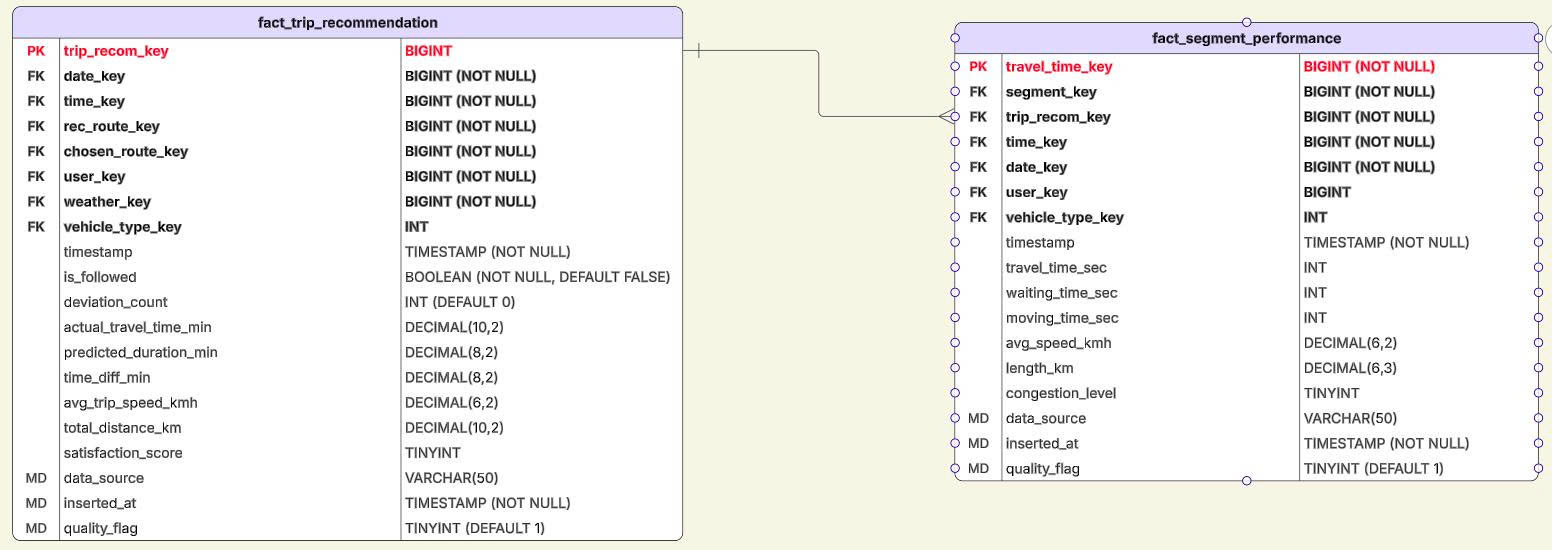
\includegraphics[width=1.0\textwidth]{Images/Picture10}
    \vspace{6mm}
    \caption{Cụm bảng fact\_trip\_recommendation và fact\_segment\_performance}
\end{figure}

\subsubsection{Bảng Dim}

\begin{figure}[H]
    \centering
    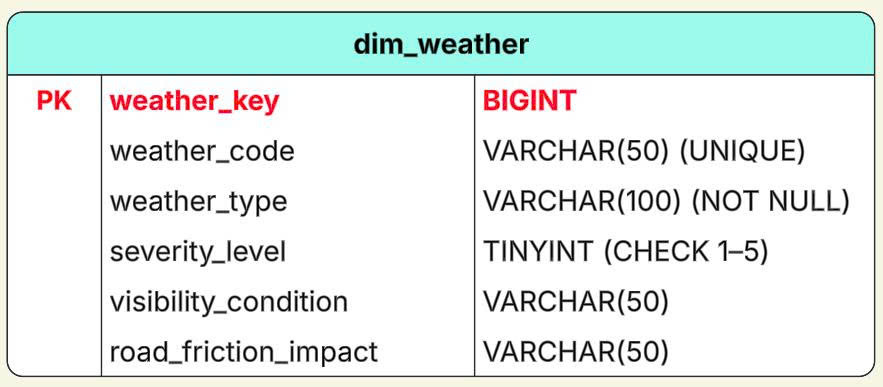
\includegraphics[width=1.0\textwidth]{Images/Picture11}
    \vspace{6mm}
    \caption{Bảng Dimension dim\_weather}
\end{figure}

\begin{figure}[H]
    \centering
    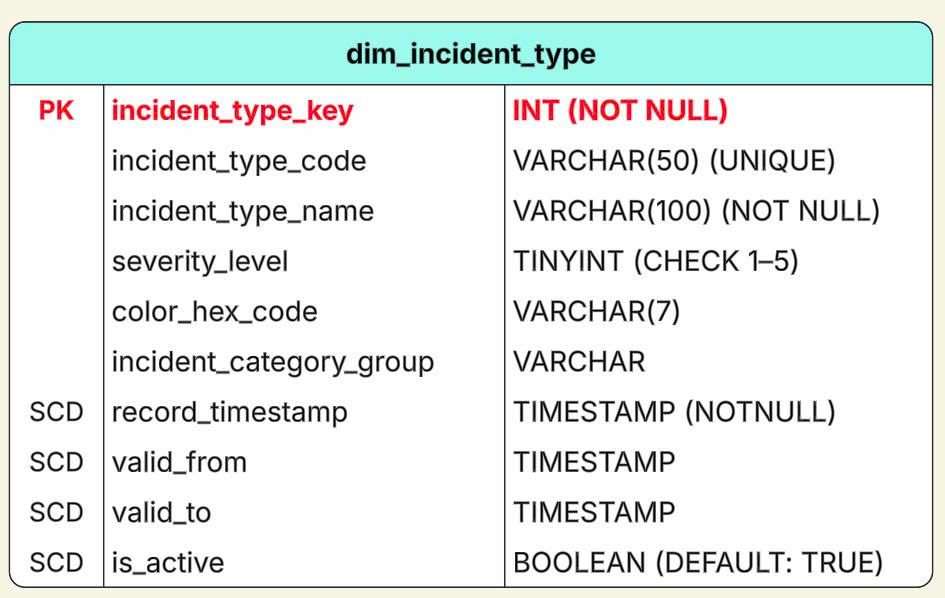
\includegraphics[width=1.0\textwidth]{Images/Picture12}
    \vspace{6mm}
    \caption{Bảng Dimension dim\_incident\_type}
\end{figure}

\begin{figure}[H]
    \centering
    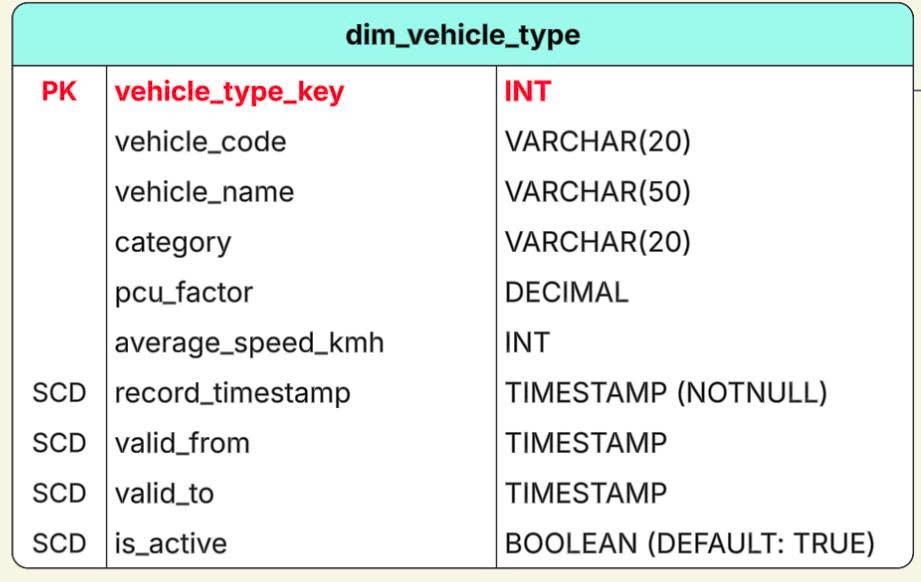
\includegraphics[width=1.0\textwidth]{Images/Picture13}
    \vspace{6mm}
    \caption{Bảng Dimension dim\_vehicle\_type}
\end{figure}

% Nhóm hình ảnh các bảng Dim liên kết (User, Time, Infrastructure)
\begin{figure}[H]
    \centering
    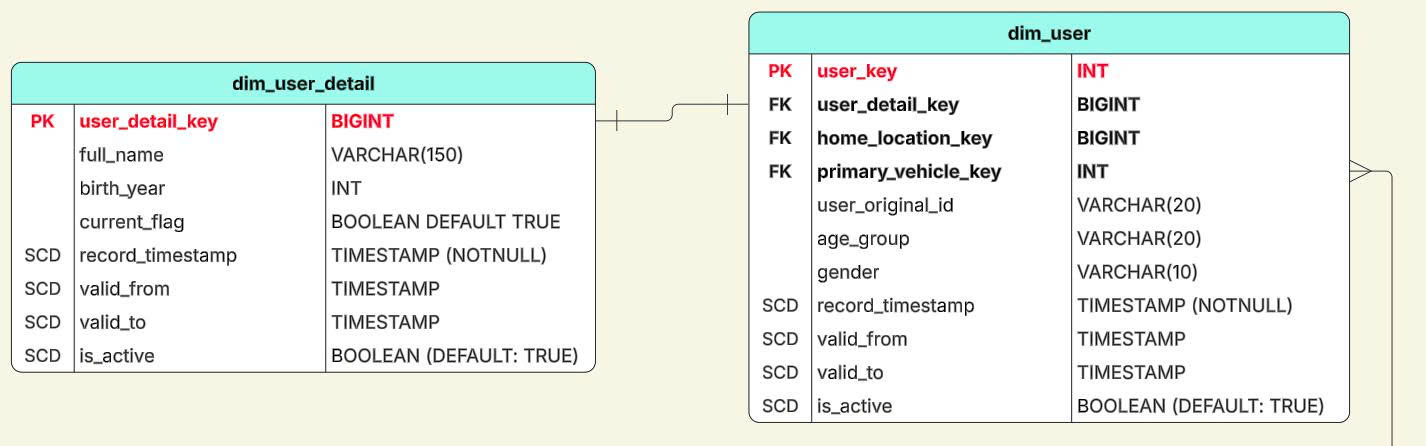
\includegraphics[width=1.0\textwidth]{Images/Picture14}
    \vspace{6mm}
    \caption{Nhóm Bảng Dimension: Người dùng}
\end{figure}

\begin{figure}[H]
    \centering
    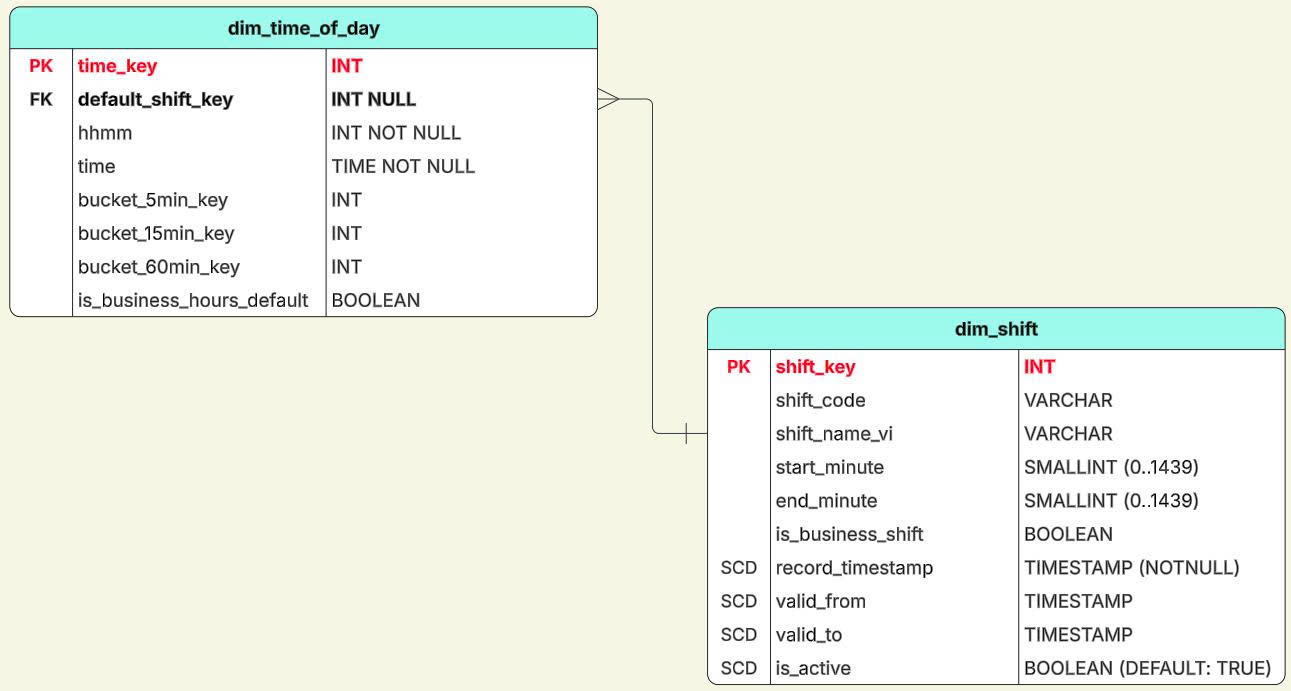
\includegraphics[width=1.0\textwidth]{Images/Picture15}
    \vspace{6mm}
    \caption{Nhóm Bảng Dimension: Thời gian (Chi tiết thời gian trong ngày)}
\end{figure}

\begin{figure}[H]
    \centering
    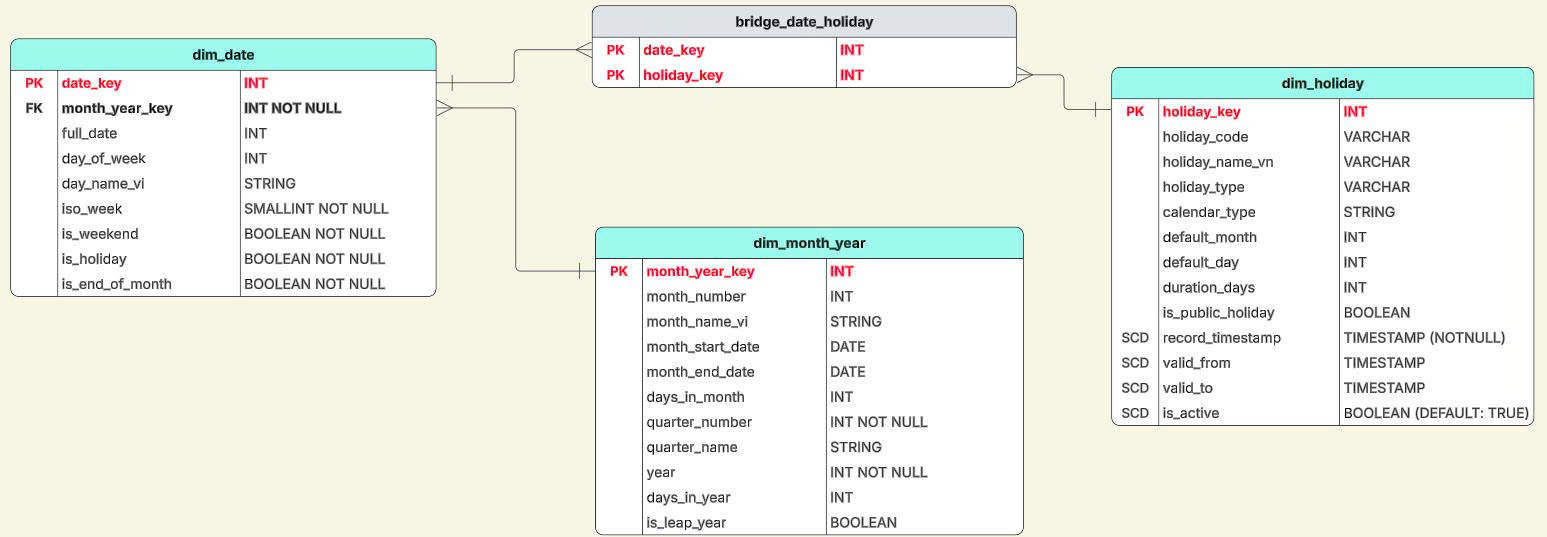
\includegraphics[width=1.0\textwidth]{Images/Picture16}
    \vspace{6mm}
    \caption{Nhóm Bảng Dimension: Thời gian (Ngày/Tháng/Năm)}
\end{figure}

\begin{figure}[H]
    \centering
    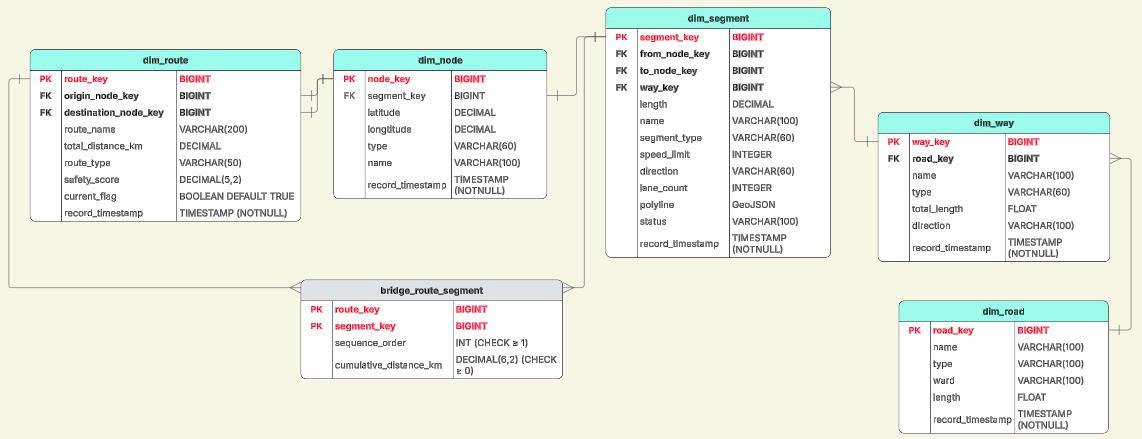
\includegraphics[width=1.0\textwidth]{Images/Picture17}
    \vspace{6mm}
    \caption{Nhóm Bảng Dimension: Hạ tầng giao thông}
\end{figure}
\subsection{Kết chương}

Chương 6 đã trình bày một cách đầy đủ tiến trình tư duy và phương pháp thiết kế kiến trúc Kho dữ liệu giao thông, thể hiện bước chuyển quan trọng từ các mô hình dữ liệu đơn giản sang một hệ kiến trúc tích hợp có tính hệ thống và đa chiều hơn.\\
Trước hết, thông qua phân tích và phản biện ở mục 5.1, nhóm nghiên cứu đã chỉ ra những hạn chế cốt lõi của việc áp dụng mô hình Lược đồ Sao rời rạc trong bối cảnh dữ liệu giao thông – nơi mà mối liên hệ giữa vận hành hạ tầng, an toàn giao thông và hành vi người dùng mang tính tương tác chặt chẽ, không thể tách biệt. Trên cơ sở đó, mô hình Galaxy Schema kết hợp với kỹ thuật chuẩn hóa chiều dạng Snowflake đã được lựa chọn và xây dựng chi tiết trong mục 5.2.\\

Thiết kế đạt được các kết quả nổi bật:
\begin{itemize}
    \item \textbf{Khắc phục phân mảnh dữ liệu:} Việc hình thành hệ thống Conformed Dimensions (như Thời gian, Segment, Phương tiện) giúp loại bỏ tình trạng rời rạc giữa các quy trình nghiệp vụ, đồng thời mở ra khả năng phân tích chéo đa lĩnh vực (cross-process analytics).
    \item \textbf{Mô hình hóa chính xác ngữ cảnh không gian:} Cấu trúc Snowflake trong nhóm chiều không gian (dim\_segment → dim\_way → dim\_road) tái hiện chính xác đặc trưng topo của mạng lưới giao thông, tạo nền tảng cho các thuật toán định tuyến, tính toán tốc độ lan truyền ùn tắc và mô phỏng sự cố.
    \item \textbf{Đáp ứng toàn diện yêu cầu nghiệp vụ:} Bốn nhóm Fact (Lưu lượng, Sự cố, Hành vi, Hiệu quả Hệ thống) bao phủ đầy đủ các nhu cầu phân tích từ giám sát thời gian thực, đánh giá vận hành, đến hỗ trợ ra quyết định chiến lược dài hạn.
\end{itemize}

Với bộ kiến trúc dữ liệu đã được định hình chắc chắn, một bài toán trọng tâm tiếp theo là xác định cách thức thu nhận dữ liệu thô từ nhiều nguồn phân tán, không đồng nhất và đưa vào hệ thống một cách nhất quán, chính xác và có khả năng mở rộng. 
